% Six replacement slides for the pigment section of BDC223 Lecture 7a.
% Match the Fira Sans / ink / teal Beamer style used for Lectures 6, 7b, 8 and 10.
% Spectra are schematic, generated from Gaussian bands, not digitised measurements.
% Approximate ether maxima: chl a 430/662 nm; chl b 453/642 nm.
% The historical taxon/pigment table follows the supplied teaching slide; see README.md.
\documentclass[aspectratio=169,11pt]{beamer}
\usepackage[sfdefault,lining]{FiraSans}
\usepackage{amsmath}
\usefonttheme{professionalfonts}
\usepackage{firamath-otf}
\setmathrm{Fira Sans}
\usepackage{tikz,pgfplots,booktabs,array,colortbl}
\pgfplotsset{compat=1.18}
\usetikzlibrary{arrows.meta,positioning,calc}
\definecolor{ink}{HTML}{1F2A37}
\definecolor{accent}{HTML}{0F766E}
\definecolor{sea}{HTML}{1D4E89}
\definecolor{grey}{HTML}{6B7280}
\definecolor{leaf}{HTML}{3F8F2F}
\definecolor{warm}{HTML}{B45309}
\definecolor{rhodo}{HTML}{B91C1C}
\definecolor{phyco}{HTML}{A03587}
\setbeamercolor{frametitle}{fg=white,bg=ink}
\setbeamercolor{normal text}{fg=ink,bg=white}
\setbeamercolor{itemize item}{fg=accent}
\setbeamertemplate{itemize item}{\small$\blacktriangleright$}
\setbeamertemplate{navigation symbols}{}
\setbeamerfont{frametitle}{size=\Large,series=\bfseries}
\setbeamertemplate{frametitle}{%
  \nointerlineskip
  \begin{beamercolorbox}[wd=\paperwidth,ht=2.4em,dp=0.9em,leftskip=1.2em]{frametitle}
    \insertframetitle
  \end{beamercolorbox}}
\setbeamertemplate{footline}{%
  \hbox to \paperwidth{\hspace{1.2em}\color{grey}\tiny BDC223 Plant Ecophysiology \textbar{} Lecture 7a: Pigments and Photosynthesis\hfill\insertframenumber\hspace{1.2em}}\vspace{0.6em}}
\setlength{\leftmargini}{1.4em}
\hyphenpenalty=10000
\newcommand{\fignote}[1]{\par\vspace{3pt}{\color{grey}\scriptsize #1}}
\newcommand{\twocol}[2]{%
  \begin{columns}[c,onlytextwidth]
    \begin{column}{0.46\textwidth}#1\end{column}
    \begin{column}{0.51\textwidth}\centering #2\end{column}
  \end{columns}}
\pgfmathdeclarefunction{ca}{1}{\pgfmathparse{exp(-((#1-430)/15)^2/2)+0.72*exp(-((#1-662)/13)^2/2)}}
\pgfmathdeclarefunction{cb}{1}{\pgfmathparse{exp(-((#1-453)/15)^2/2)+0.55*exp(-((#1-642)/14)^2/2)}}
\pgfmathdeclarefunction{carot}{1}{\pgfmathparse{0.78*exp(-((#1-449)/17)^2/2)+0.65*exp(-((#1-477)/13)^2/2)}}
\pgfmathdeclarefunction{pe}{1}{\pgfmathparse{0.24*exp(-((#1-498)/18)^2/2)+0.58*exp(-((#1-542)/14)^2/2)+0.81*exp(-((#1-565)/13)^2/2)}}
\pgfmathdeclarefunction{pc}{1}{\pgfmathparse{exp(-((#1-620)/23)^2/2)}}
\pgfplotsset{spectral/.style={
  width=13.5cm,height=5.2cm,xmin=400,xmax=700,ymin=0,ymax=1.18,
  domain=400:700,samples=301,axis lines=left,
  xlabel={Wavelength (nm)},ylabel={Relative absorption},
  xtick={400,450,500,550,600,650,700},ytick={0,0.5,1},
  tick label style={font=\footnotesize},label style={font=\small},
  grid=major,grid style={grey!13},
  legend style={font=\footnotesize,draw=none,fill=white,at={(0.5,1.04)},anchor=south,legend columns=2},
  legend cell align=left}}

\begin{document}

% 1: replaces BDC223_L06a_slide03.jpeg.
\begin{frame}{Chlorophyll and accessory pigments}
\twocol{
\begin{itemize}
  \item Pigments absorb light at different wavelengths
  \item Accessory pigments transfer excitation energy to chlorophyll-\textit{a}
  \item Reaction-centre chlorophyll-\textit{a} starts electron transfer in plants and most algae
  \item Pigments and proteins form organised light-harvesting complexes
\end{itemize}}{
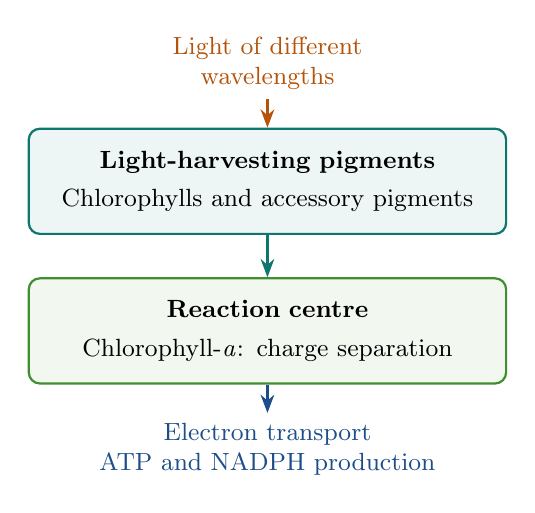
\begin{tikzpicture}[font=\small,>=Stealth]
  \node[align=center,text=warm] (light) at (0,2.4) {Light of different\\wavelengths};
  \node[draw=accent,thick,rounded corners,fill=accent!7,text width=5.5cm,align=center,inner sep=8pt] (antenna) at (0,0.9)
    {\textbf{Light-harvesting pigments}\\[3pt]Chlorophylls and accessory pigments};
  \node[draw=leaf,thick,rounded corners,fill=leaf!7,text width=5.5cm,align=center,inner sep=8pt] (rc) at (0,-1.0)
    {\textbf{Reaction centre}\\[3pt]Chlorophyll-\textit{a}: charge separation};
  \node[align=center,text=sea] (output) at (0,-2.5) {Electron transport\\ATP and NADPH production};
  \draw[->,thick,warm] (light) -- (antenna);
  \draw[->,thick,accent] (antenna) -- (rc);
  \draw[->,thick,sea] (rc) -- (output);
\end{tikzpicture}}
\end{frame}

% 2: replaces BDC223_L06a_slide04.jpeg.
\begin{frame}{Absorption by chlorophylls a and b}
\centering
\begin{tikzpicture}
\begin{axis}[spectral,legend columns=2]
  \addplot[rhodo,very thick] {ca(x)};
  \addlegendentry{Chlorophyll \textit{a}}
  \addplot[leaf,very thick,dashed] {cb(x)};
  \addlegendentry{Chlorophyll \textit{b}}
  \draw[grey,dotted] (axis cs:430,0) -- (axis cs:430,1);
  \draw[grey,dotted] (axis cs:662,0) -- (axis cs:662,0.72);
  \node[font=\scriptsize,text=rhodo,anchor=south east] at (axis cs:428,1.02) {430 nm};
  \node[font=\scriptsize,text=leaf,anchor=south west] at (axis cs:455,1.02) {453 nm};
  \node[font=\scriptsize,text=leaf,anchor=south east] at (axis cs:638,0.57) {642 nm};
  \node[font=\scriptsize,text=rhodo,anchor=south west] at (axis cs:664,0.75) {662 nm};
\end{axis}
\end{tikzpicture}
\fignote{Schematic spectra in diethyl ether; each curve has its own relative scale. Peaks shift when pigments bind to proteins in living cells.}
\end{frame}

% 3: replaces BDC223_L06a_slide05.jpeg.
\begin{frame}{The green gap}
\centering
\begin{tikzpicture}
\begin{axis}[spectral,height=5.25cm,ymax=1.16,legend style={at={(0.5,1.03)},anchor=south}]
  \fill[leaf!12] (axis cs:500,0) rectangle (axis cs:600,1.12);
  \addplot[leaf!70!black,very thick] {ca(x)};
  \addlegendentry{Chlorophyll \textit{a}, schematic}
  \node[font=\small,text=accent,align=center] at (axis cs:550,0.64) {\textbf{Green gap}\\[3pt]Weak absorption};
  \node[font=\footnotesize,text=sea,align=center] at (axis cs:470,0.90) {Blue\\peak};
  \node[font=\footnotesize,text=rhodo,align=center] at (axis cs:652,1.0) {Red\\peak};
\end{axis}
\end{tikzpicture}
\fignote{Chlorophyll absorbs less strongly in the green region. Reflected and transmitted green light contributes to the colour of leaves and green algae.}
\end{frame}

% 4: replaces BDC223_L06a_slide06.jpeg.
\begin{frame}{Accessory pigments extend light absorption}
\centering
\begin{tikzpicture}
\begin{axis}[spectral,height=4.7cm,ymax=1.2,
  legend style={font=\scriptsize,at={(0.5,1.05)},anchor=south,legend columns=3,draw=none,fill=white},
  legend cell align=left]
  \addplot[rhodo,thick] {ca(x)}; \addlegendentry{Chlorophyll \textit{a}}
  \addplot[leaf,thick,dashed] {cb(x)}; \addlegendentry{Chlorophyll \textit{b}}
  \addplot[warm,very thick,densely dotted] {carot(x)/1.04}; \addlegendentry{$\beta$-carotene}
  \addplot[phyco,very thick,dashdotted] {pe(x)/0.99}; \addlegendentry{Phycoerythrin}
  \addplot[sea,very thick] {pc(x)}; \addlegendentry{Phycocyanin}
\end{axis}
\end{tikzpicture}
\fignote{Illustrative profiles, each scaled independently. Carotenoids mainly absorb blue to blue-green light; phycobiliproteins extend absorption into green, yellow and orange wavelengths.}
\end{frame}

% 5: replaces BDC223_L06a_slide07.jpeg.
\begin{frame}{Three main pigment classes}
\fontsize{9.3}{11.5}\selectfont
\renewcommand{\arraystretch}{1.20}
\begin{tabular}{@{}>{\raggedright\arraybackslash}p{2.8cm}>{\raggedright\arraybackslash}p{4.4cm}>{\raggedright\arraybackslash}p{5.95cm}@{}}
\toprule
\textbf{Class} & \textbf{Examples} & \textbf{Main roles}\\
\midrule
\textcolor{leaf}{\textbf{Chlorophylls}} & Chlorophylls \textit{a}, \textit{b} and \textit{c} & Light harvesting; chlorophyll-\textit{a} also drives photochemistry\\
\textcolor{warm}{\textbf{Carotenoids}} & Carotenes: $\beta$-carotene\newline Xanthophylls: fucoxanthin, lutein & Light harvesting and protection against excess light\\
\textcolor{phyco}{\textbf{Phycobilins}} & Protein-bound pigments in phycoerythrin and phycocyanin & Light harvesting in red algae, cyanobacteria and cryptophytes\\
\bottomrule
\end{tabular}
\vspace{0.2cm}
\begin{itemize}
  \item More than forty pigments occur across photoautotrophs
  \item Binding to different proteins can shift a pigment's absorption spectrum
\end{itemize}
\end{frame}

% 6: replaces BDC223_L06a_slide08.jpeg. Preserve all nine historical group rows.
\begin{frame}{Pigments in different algal groups}
\fontsize{8.1}{10}\selectfont
\renewcommand{\arraystretch}{1.28}
\setlength{\tabcolsep}{5pt}
\begin{tabular}{@{}>{\raggedright\arraybackslash}p{3.0cm}>{\raggedright\arraybackslash}p{10.64cm}@{}}
\rowcolor{accent!15}\textbf{Algal group} & \textbf{Examples of reported pigments}\\
\addlinespace[2pt]
Bacillariophyceae & Chl \textit{a}, \textit{c}; $\beta$-carotene; fucoxanthin; diatoxanthin; diadinoxanthin\\
\rowcolor{ink!4}Dinophyceae & Chl \textit{a}, \textit{c}$_2$; $\beta$-carotene; peridinin; neoperidinin\\
Phaeophyceae & Chl \textit{a}, \textit{c}$_1$, \textit{c}$_2$; $\beta$-carotene; fucoxanthin\\
\rowcolor{ink!4}Raphidophyceae & Chl \textit{a}, \textit{c}; diatoxanthin; diadinoxanthin; heteroxanthin; fucoxanthin\\
Cryptophyceae & Chl \textit{a}, \textit{c}$_2$; $\alpha$-carotene; diatoxanthin; phycoerythrin; phycocyanin\\
\rowcolor{ink!4}Euglenophyceae & Chl \textit{a}, \textit{b}; $\beta$-carotene; astaxanthin; antheraxanthin; diadinoxanthin; neoxanthin\\
Chlorophyceae & Chl \textit{a}, \textit{b}; $\alpha$-, $\beta$- and $\gamma$-carotene; lutein; siphonaxanthin; siphonein\\
\rowcolor{ink!4}Charophyceae & Chl \textit{a}, \textit{b}; $\alpha$-, $\beta$- and $\gamma$-carotene; various xanthophylls\\
Prasinophyceae & Chl \textit{a}, \textit{b}; $\beta$-carotene; siphonaxanthin; siphonein\\
\bottomrule
\end{tabular}
\fignote{After South and Whittick (1987). Pigment combinations vary among species; these are not universal diagnostic lists. Chl = chlorophyll.}
\end{frame}

\end{document}
